\section{Implementation of Perturb and Observe algorithm}\label{MPPTImplementation}

Things to write in this section: 
\begin{itemize}
	\item Why we use duty cycle as output of the MPPT instead of a voltage ref. 
	\item Frequency of the MPPT algorithm is 100Hz. Every 10ms the MPPT evaluates voltage and power to decide if it is necessary to increase or decrease D. 
	\item Initial conditions: enable the MPPT after 5Ts (50ms) to ensure that Vin has reached the open circuit voltage, counter = 5 to have some open loop measurements before starting the voltage evaluation, the system starts in buck mode (D=0.25) with fix variations of duty cycle (0.01), limits of duty cycle 0.05<D<0.95 to avoid problems in buck and in boost mode respetively. 
	\item The current measurement is carried out in the inductor instead of in the panel so it is possible to implement future PI control loops to improve the MPPT algorithm. For this reason it's necessary to make a transformation of this current in the case of buck mode (multiplying by the corresponding duty cycle, Dbuck = 2*D). However in boost mode it's not necessary because the panel current is the same as the inductor's current. 
	\item Mode decision is done by mapping the transfer functions (refer to Figures) corresponding to buck and boost mode and including an extra block after the MPPT which has as input the value of D and returns the duty cycle for buck or boost mode. This duty cycles are used to generate the corresponding PWM signals according to the mode the converter is working at each time. 
	\item Also mention the case when a change in irradiance takes place it's a good idea to reset the value of delta D to 0.01. This is because we are using variable step and when the system detects the change in irradiance it will keep the corresponding value of delta D which will be very small because the system already could have reached the MPP (variable step). 
	\item The MPPT algorithm is an improved version of the simple one explained in the previous section as it reduces the duty cycle step/increment by 2 iteractively when it detects it has reached the MPP.

\end{itemize}


\begin{figure}[H]
	\begin{minipage}[b]{0.8\linewidth}
		\centering
		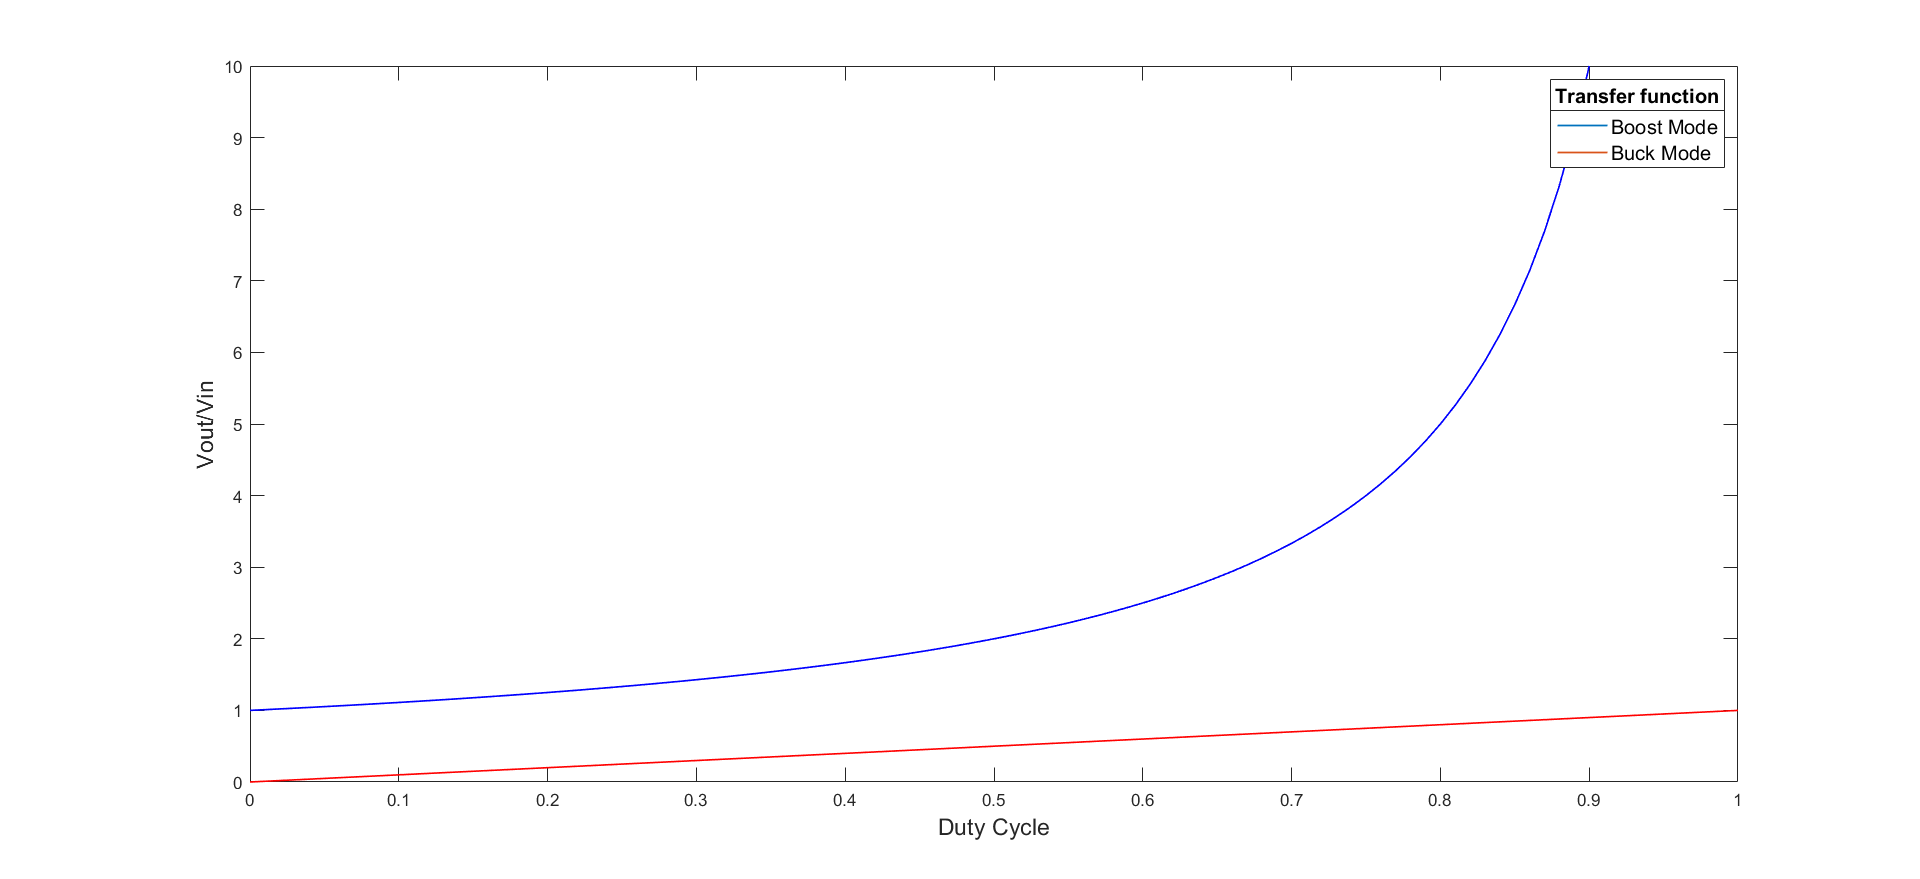
\includegraphics[width=\textwidth]{../Pictures/transfer_function_buck_boost_mode}
		\caption{Transfer function of buck mode and boost mode.}
		\label{fig:tfmodes}
	\end{minipage}
	\hspace{0.5cm}
	\begin{minipage}[b]{0.8\linewidth}
		\centering
		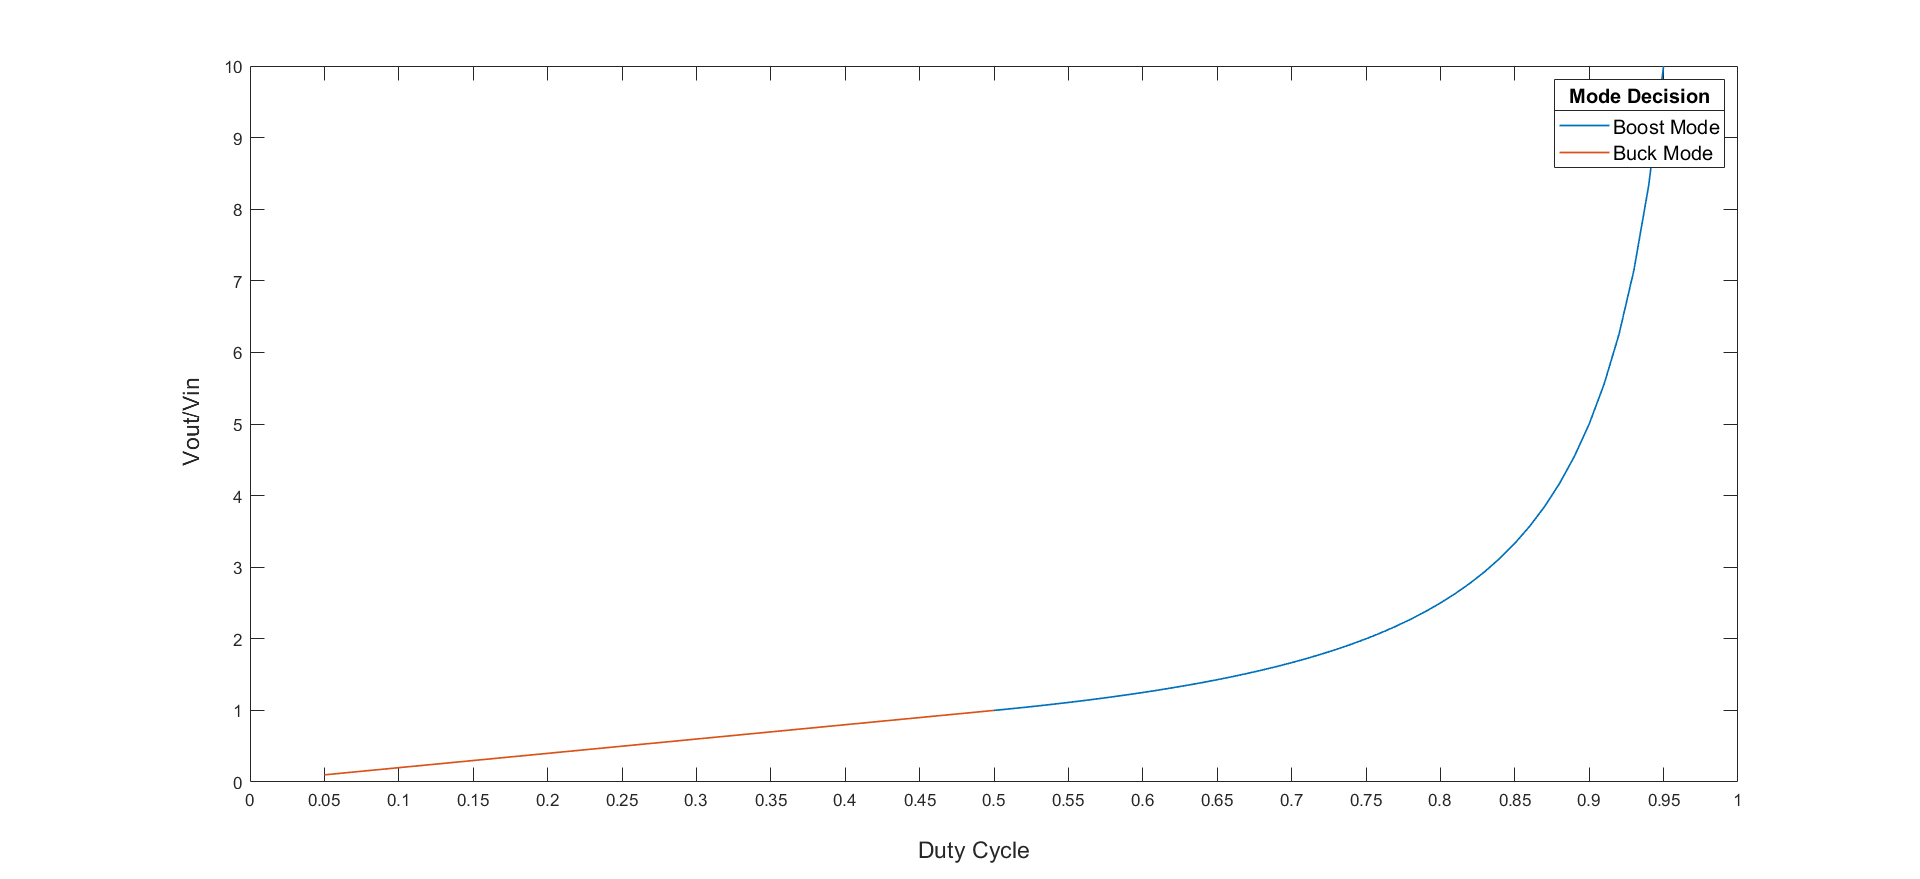
\includegraphics[width=\textwidth]{../Pictures/Mode_decision_duty_vs_gain}
		\caption{Mapping to decide the mode of operation.}
		\label{fig:modedecisionmapping}
	\end{minipage}
\end{figure}


\begin{figure}[H]
	\begin{center}
		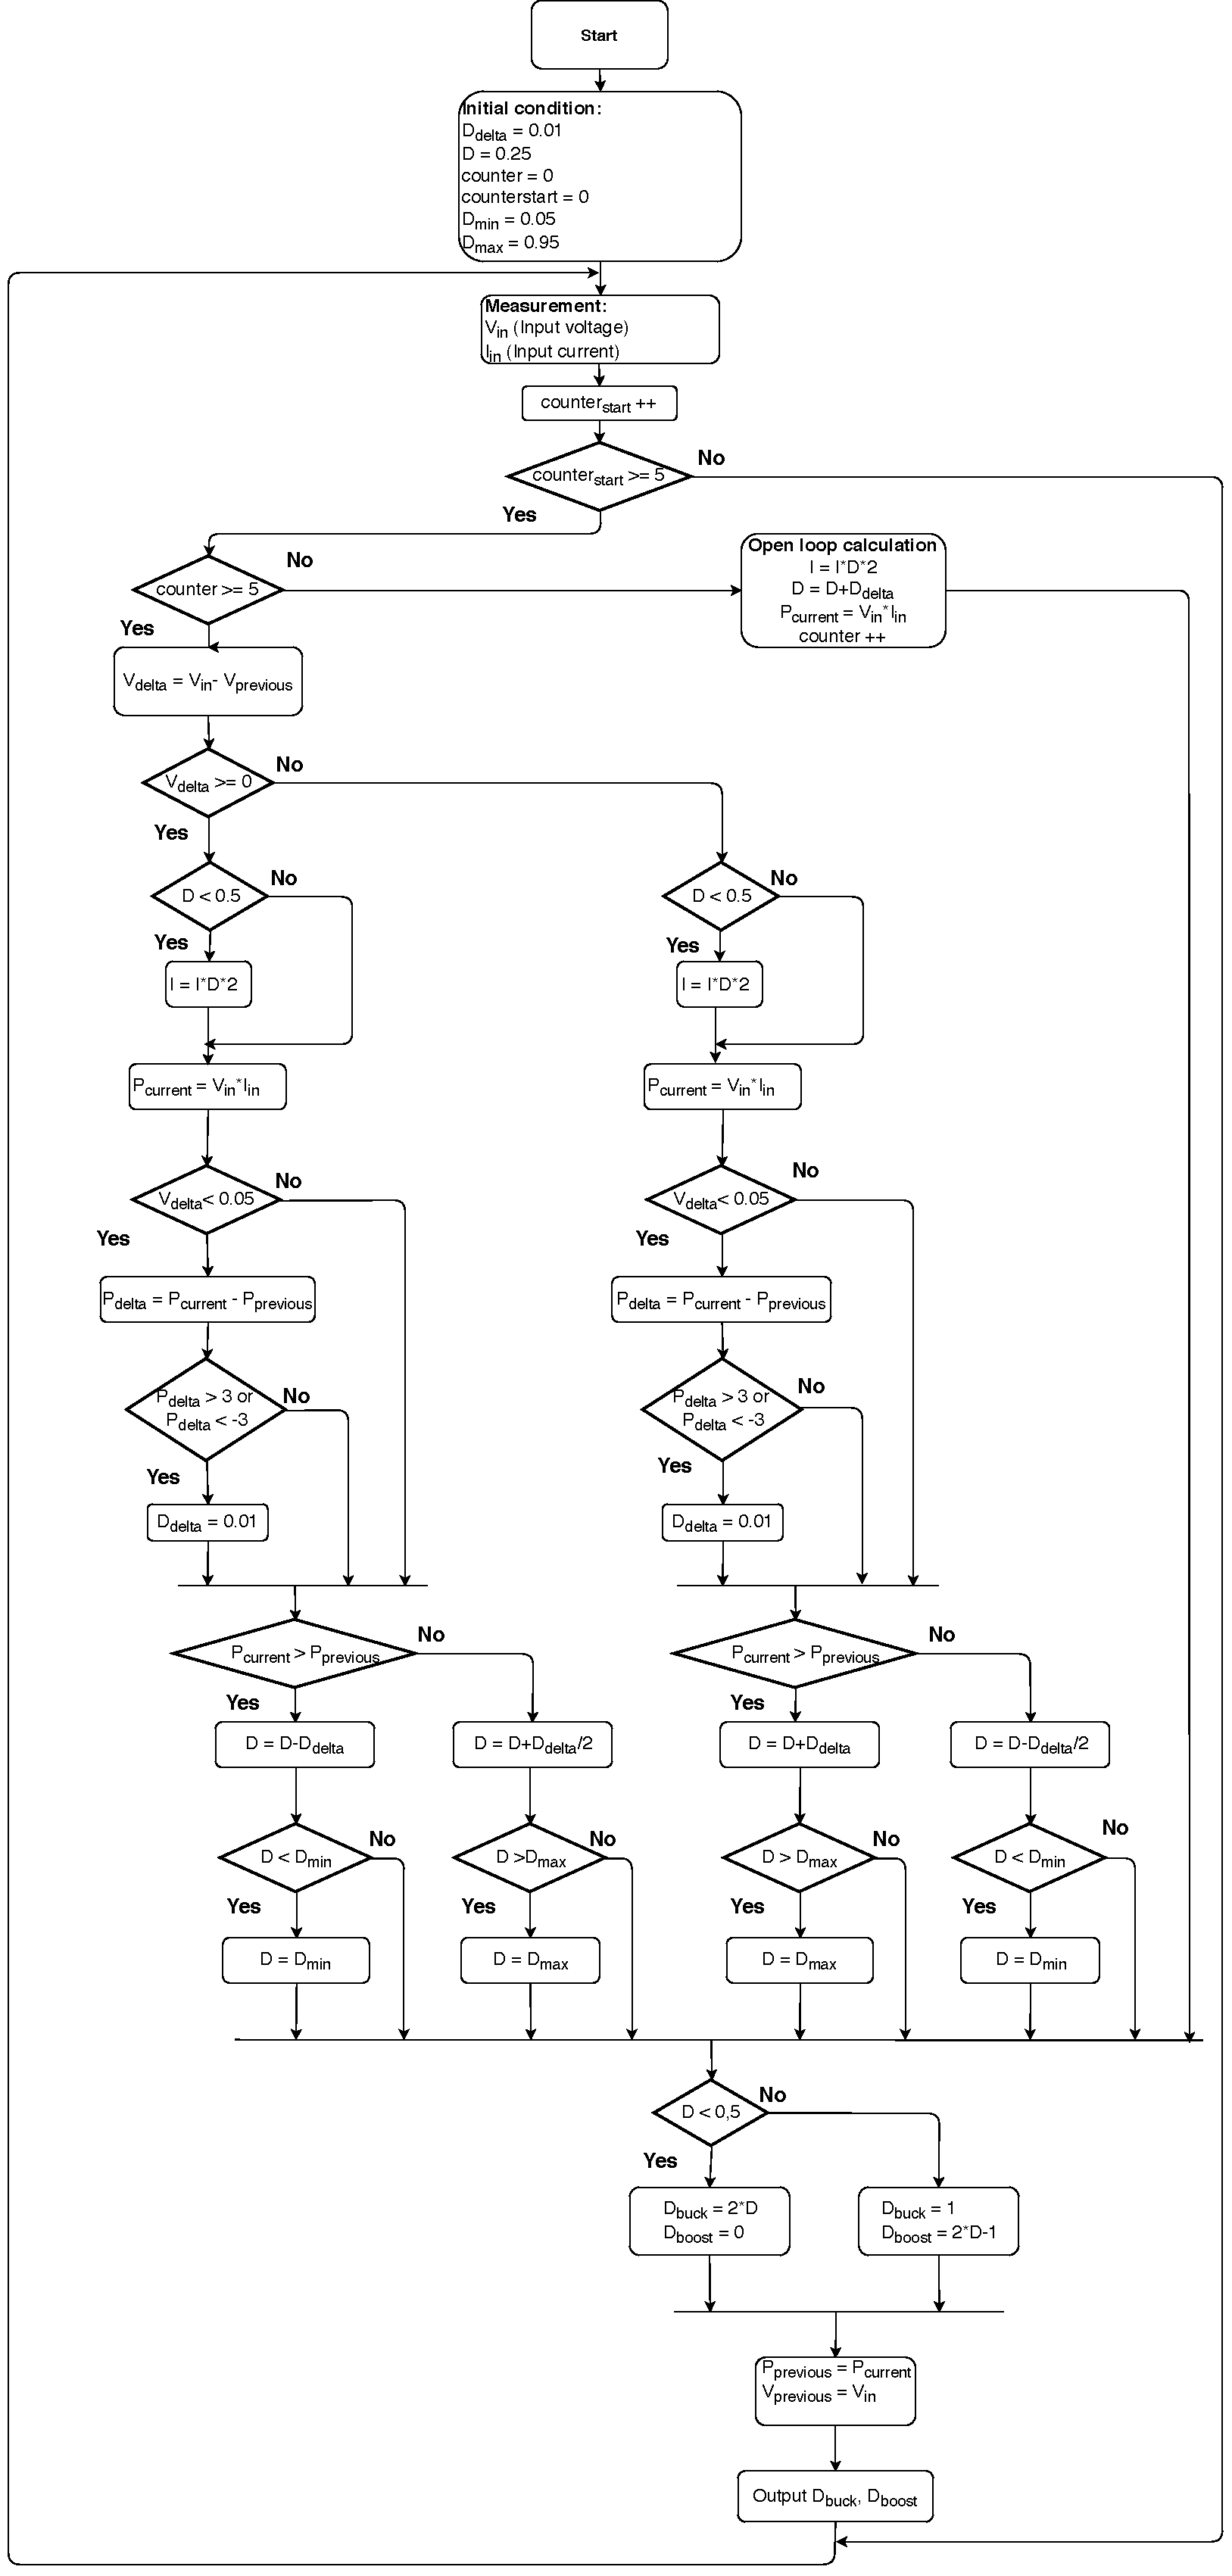
\includegraphics[width=0.75\textwidth]{../Pictures/P1/Flow_chart/2018_11_15_Flow_chart_MPPT_Buck-Boost_converter}
		\caption{flow chart final }
		\label{fcfinal}
	\end{center}	
\end{figure}
